% ### Erste Seite der Navier-Stokes-Gleichungen ###
\centering
\section*{\myul{Navier-Stokes-Gleichungen}}

\begin{tikzpicture}[remember picture, overlay]

% --- ERSTE REIHE: Am Seitenursprung anfangen
\setlength{\rowheight}{35mm}

    % A1) Erste Kachel relativ zum Seitenursprung
    \setlength{\cellwidth}{95mm}
    \Tile{A1}{([xshift=10mm, yshift=-20mm]current page.north west)}{\cellwidth}{\rowheight}
        {
            \vspace{-\TileSep}
            \titlebf{Scherraten-Tensor}\\ \vspace{-4mm}
            \begin{equation*}
                \underline{\underline{D}} = 
                \left(
                \begin{matrix}
                    \dfrac{\partial u}{\partial x} & \dfrac{1}{2}\left(\dfrac{\partial u}{\partial y}+\dfrac{\partial v}{\partial x}\right) & \dfrac{1}{2}\left(\dfrac{\partial u}{\partial z}+\dfrac{\partial w}{\partial x}\right) \\[2.0ex]
                    \dfrac{1}{2}\left(\dfrac{\partial u}{\partial y}+\dfrac{\partial v}{\partial x}\right) & \dfrac{\partial v}{\partial y} & \dfrac{1}{2}\left(\dfrac{\partial v}{\partial z}+\dfrac{\partial w}{\partial y}\right) \\[2.0ex]
                    \dfrac{1}{2}\left(\dfrac{\partial u}{\partial z}+\dfrac{\partial w}{\partial x}\right) & \dfrac{1}{2}\left(\dfrac{\partial v}{\partial z}+\dfrac{\partial w}{\partial y}\right) & \dfrac{\partial w}{\partial z}
                \end{matrix}
                \right)
            \end{equation*}
        }{0}{1}{1}{0}

    % B1) Zweite Kachel rechts anbauen
    \setlength{\cellwidth}{95mm}
    \Tile{B1}{(A1.north east)}{\cellwidth}{\rowheight}
        {
            \vspace{-\TileSep}
            \titlebf{Drehgeschwindigkeits-Tensor}\\ \vspace{-4mm}
            \begin{equation*}
                \underline{\underline{W}} = 
                \left(
                \begin{matrix}
                    0 & \dfrac{1}{2}\left(\dfrac{\partial u}{\partial y}-\dfrac{\partial v}{\partial x}\right) & \dfrac{1}{2}\left(\dfrac{\partial u}{\partial z}-\dfrac{\partial w}{\partial x}\right) \\[2.0ex]
                    \dfrac{1}{2}\left(\dfrac{\partial v}{\partial x}-\dfrac{\partial u}{\partial y}\right) & 0 & \dfrac{1}{2}\left(\dfrac{\partial v}{\partial z}-\dfrac{\partial w}{\partial y}\right) \\[2.0ex]
                    \dfrac{1}{2}\left(\dfrac{\partial w}{\partial x}-\dfrac{\partial u}{\partial z}\right) & \dfrac{1}{2}\left(\dfrac{\partial w}{\partial y}-\dfrac{\partial v}{\partial z}\right) & 0
                \end{matrix}
                \right)
            \end{equation*}
        }{0}{0}{1}{0}

% --- ZWEITE REIHE: Unten anbauen
\setlength{\rowheight}{36.5mm}

    % A2) Erste Kachel unten anbauen
    \setlength{\cellwidth}{190mm}
    \Tile{A2}{(A1.south west)}{\cellwidth}{\rowheight}
        {
            \titlebf{Spannungs-Tensor}\\ \vspace{-4mm}
            \begin{equation*}
                \underline{\underline{\sigma}} = \left(
                \begin{matrix}
                    -p+2\,\eta\left(\dfrac{\partial u}{\partial x} - \dfrac{1}{3}\,\text{div}\!\left(\underline{v}\right)\right) & \eta\left(\dfrac{\partial u}{\partial y} + \dfrac{\partial v}{\partial x}\right) & \eta\left(\dfrac{\partial u}{\partial z} + \dfrac{\partial w}{\partial x}\right) \\[2.0ex]
                    \eta\left(\dfrac{\partial v}{\partial x} + \dfrac{\partial u}{\partial y}\right) & -p+2\,\eta\left(\dfrac{\partial v}{\partial y} - \dfrac{1}{3}\,\text{div}\!\left(\underline{v}\right)\right) & \eta\left(\dfrac{\partial v}{\partial z} + \dfrac{\partial w}{\partial y}\right) \\[2.0ex]
                    \eta\left(\dfrac{\partial w}{\partial x} + \dfrac{\partial u}{\partial z}\right) & \eta\left(\dfrac{\partial w}{\partial y} + \dfrac{\partial v}{\partial z}\right) & -p+2\,\eta\left(\dfrac{\partial w}{\partial z} - \dfrac{1}{3}\,\text{div}\!\left(\underline{v}\right)\right)
                \end{matrix}
                \right) \hspace{4.5mm}
            \end{equation*}
        }{0}{0}{1}{0}

% --- DRITTE REIHE: Unten anbauen
\setlength{\rowheight}{19mm}

    % A3) Erste Kachel relativ zum Seitenursprung
    \setlength{\cellwidth}{95mm}
    \Tile{A3}{(A2.south west)}{\cellwidth}{\rowheight}
        {
            \titlebf{Divergenz des Spannungstensors}\\ \vspace{-2.5mm}
            \begin{equation*}
                \text{div}\!\left(\underline{\underline{\sigma}}\right) = -\nabla(p) + 2\,\text{div}\!\left(\eta\,\underline{\underline{D}}\right) - \frac{2}{3}\,\nabla\!\left(\eta\,\text{div}\!\left(\underline{v}\right)\right)
            \end{equation*}
        }{0}{1}{1}{0}

    % B3) Zweite Kachel rechts anbauen
    \setlength{\cellwidth}{95mm}
    \Tile{B3}{(A3.north east)}{\cellwidth}{\rowheight}
        {
            \titlebf{Inkompressible Strömung}\\ \vspace{-3.5mm}
            \begin{equation*}
                \frac{\partial\underline{v}}{\partial t} + \underline{v} \cdot \nabla\!\left(\underline{v}\right) = -\nabla\!\left(\frac{p}{\rho}\right) + \nu\Delta\!\left(\underline{v}\right) + \underline{f}
            \end{equation*}
        }{0}{0}{1}{0}

% --- VIERTE REIHE: Unten anbauen
\setlength{\rowheight}{40mm}

    % A4) Erste Kachel unten anbauen
    \setlength{\cellwidth}{190mm}
    \Tile{A4}{(A3.south west)}{\cellwidth}{\rowheight}
        {
            \titlebf{Kartesische Koordinaten (Newton'sche Fluide)}\\ \vspace{-4mm}
            \begin{align*}
                \rho\left[\frac{\partial u}{\partial t} + u\,\frac{\partial u}{\partial x} + v\,\frac{\partial u}{\partial y} + w\,\frac{\partial u}{\partial z}\right] &=
                -\frac{\partial p}{\partial x} + \rho\,f_x
                + \frac{\partial}{\partial x}\left[2\,\eta\left(\frac{\partial u}{\partial x}-\frac{\text{div}\!\left(\underline{v}\right)}{3}\right)\right]
                + \frac{\partial}{\partial y}\left[\eta\left(\frac{\partial u}{\partial y}+\frac{\partial v}{\partial x}\right)\right]
                + \frac{\partial}{\partial z}\left[\eta\left(\frac{\partial u}{\partial z}+\frac{\partial w}{\partial x}\right)\right] \\[0.25ex]
                \rho\left[\frac{\partial v}{\partial t} + u\,\frac{\partial v}{\partial x} + v\,\frac{\partial v}{\partial y} + w\,\frac{\partial v}{\partial z}\right] &=
                -\frac{\partial p}{\partial y} + \rho\,f_y
                + \frac{\partial}{\partial x}\left[\eta\left(\frac{\partial v}{\partial x}+\frac{\partial u}{\partial y}\right)\right]
                + \frac{\partial}{\partial y}\left[2\,\eta\left(\frac{\partial v}{\partial y}-\frac{\text{div}\!\left(\underline{v}\right)}{3}\right)\right]
                + \frac{\partial}{\partial z}\left[\eta\left(\frac{\partial v}{\partial z}+\frac{\partial w}{\partial y}\right)\right] \\[0.25ex]
                \rho\left[\frac{\partial w}{\partial t} + u\,\frac{\partial w}{\partial x} + v\,\frac{\partial w}{\partial y} + w\,\frac{\partial w}{\partial z}\right] &=
                -\frac{\partial p}{\partial z} + \rho\,f_z
                + \frac{\partial}{\partial x}\left[\eta\left(\frac{\partial w}{\partial x}+\frac{\partial u}{\partial z}\right)\right]
                + \frac{\partial}{\partial y}\left[\eta\left(\frac{\partial w}{\partial y}+\frac{\partial v}{\partial z}\right)\right]
                + \frac{\partial}{\partial z}\left[2\,\eta\left(\frac{\partial w}{\partial z}-\frac{\text{div}\!\left(\underline{v}\right)}{3}\right)\right]
            \end{align*}
        }{0}{0}{1}{0}

% --- FÜNFTE REIHE: Unten anbauen
\setlength{\rowheight}{38.5mm}

    % A5) Erste Kachel unten anbauen
    \setlength{\cellwidth}{190mm}
    \Tile{A5}{(A4.south west)}{\cellwidth}{\rowheight}
        {
            \titlebf{Kartesische Koordinaten (Inkompressible Fluide)}\\ \vspace{-4mm}
            \begin{align*}
                \frac{\partial u}{\partial t} + u\,\frac{\partial u}{\partial x} + v\,\frac{\partial u}{\partial y} + w\,\frac{\partial u}{\partial z} &=
                -\frac{1}{\rho}\,\frac{\partial p}{\partial x} + \nu\left(\frac{\partial^2 u}{\partial x^2} + \frac{\partial^2 u}{\partial y^2} + \frac{\partial^2 u}{\partial z^2}\right) + f_x \\
                \frac{\partial v}{\partial t} + u\,\frac{\partial v}{\partial x} + v\,\frac{\partial v}{\partial y} + w\,\frac{\partial v}{\partial z} &=
                -\frac{1}{\rho}\,\frac{\partial p}{\partial y} + \nu\left(\frac{\partial^2 v}{\partial x^2} + \frac{\partial^2 v}{\partial y^2} + \frac{\partial^2 v}{\partial z^2}\right) + f_y \\
                \frac{\partial w}{\partial t} + u\,\frac{\partial w}{\partial x} + v\,\frac{\partial w}{\partial y} + w\,\frac{\partial w}{\partial z} &=
                -\frac{1}{\rho}\,\frac{\partial p}{\partial z} + \nu\left(\frac{\partial^2 w}{\partial x^2} + \frac{\partial^2 w}{\partial y^2} + \frac{\partial^2 w}{\partial z^2}\right) + f_z
            \end{align*}
        }{0}{0}{1}{0}

% --- SECHSTE REIHE: Unten anbauen
\setlength{\rowheight}{90mm}

    % A6) Erste Kachel relativ zum Seitenursprung
    \setlength{\cellwidth}{55mm}
    \Tile{A6}{(A5.south west)}{\cellwidth}{\rowheight}
        {
            \titlebf{Couette-Viskosimeter}\\ \vspace{-4mm}
            \begin{equation*}
                u = U\,\frac{y}{h}
            \end{equation*}%
            \vspace{-5mm}
            \begin{minipage}[t]{0.5\cellwidth-\TileSep}
                \centering
                \vspace{-3mm}
                \begin{equation*}
                    \tau_\text{W} = \frac{M_h}{2\,\pi\,r_0^2\,b}
                \end{equation*}%
                \vspace{-2.5mm}
                \begin{equation*}
                    \dot{\gamma} = \frac{u_\text{W}}{h}
                \end{equation*}%
                \vspace{-1.5mm}
            \end{minipage}%
            \vline
            \begin{minipage}[t]{0.5\cellwidth-\TileSep}
                \centering
                \vspace{-2mm}
                \begin{equation*}
                    \eta = \frac{\tau_\text{W}}{\dot{\gamma}}
                \end{equation*}%
                \vspace{-2.5mm}
                \begin{equation*}
                    \nu = \frac{\eta}{\rho} = \frac{\tau_\text{W}}{\rho\,\dot{\gamma}}
                \end{equation*}%
                \vspace{-1.5mm}
            \end{minipage}%
            \vspace{-1.8mm}
            {%
            \scriptsize
            \begin{align*}
                M_\text{h}   &= \text{Haltemoment}             \\[-0.5ex]
                \dot{\gamma} &= \text{Schergeschwindigkeit}    \\[-0.5ex]
                \eta         &= \text{Dynamische Viskosität}   \\[-0.5ex]
                \nu          &= \text{Kinematische Viskosität}
            \end{align*}
            }%
            \vspace{-4mm}\\
            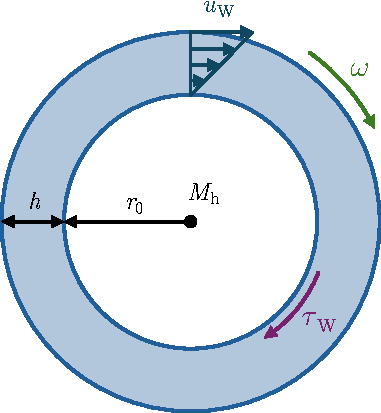
\includegraphics[width=0.7\cellwidth]{images/couette-strömung.pdf}
        }{0}{1}{0}{0}

    % B6) Zweite Kachel rechts anbauen
    \setlength{\cellwidth}{135mm}
    \Tile{B6}{(A6.north east)}{\cellwidth}{\rowheight}
        {
            \titlebf{Gesetz von Hagen-Poiseuille}\\ \vspace{1mm}
            \begin{minipage}[t]{0.6\cellwidth-\TileSep}
                \centering
                \titlerm{Radialgeschwindigkeit}\\ \vspace{-4mm}
                \begin{equation*}
                    w = \frac{a}{4}\left(r^2-R^2\right) = w_\text{max}\left(1-\frac{r^2}{R^2}\right)
                \end{equation*}%
                \vspace{-3mm}\\
                \hspace{-\TileSep}\rule{\dimexpr\textwidth-\TileSep}{0.5pt} \\ \vspace{0.5mm}
                \begin{minipage}[t]{0.58\textwidth}
                    \centering
                    \titlerm{Massenstrom}\\ \vspace{-4mm}
                    \begin{equation*}
                        \resizebox{\textwidth-2\TileSep}{!}{%
                        $\dot{m} = \dfrac{1}{2}\,\rho\,\pi\,w_\text{max}\,R^2 = \rho\,\pi\,R^2\,\overline{w}$
                        }
                    \end{equation*}
                \end{minipage}%
                \vline
                \begin{minipage}[t]{0.42\textwidth}
                    \centering
                    \titlerm{Reynoldszahl}\\ \vspace{-4mm}
                    \begin{equation*}
                        \resizebox{\textwidth-2\TileSep}{!}{%
                        $\mathrm{Re}_D = \dfrac{\rho\,\overline{w}\,D}{\eta} = \dfrac{\overline{w}\,D}{\nu}$
                        }
                    \end{equation*}%
                    \vspace{-3.5mm}
                \end{minipage}%
                \vspace{1.6mm}\\
                \hspace{-\TileSep}\rule{\dimexpr\textwidth-\TileSep}{0.5pt} \\ \vspace{0.5mm}
                \titlerm{Druckdifferenz}\\ \vspace{-4mm}
                \begin{equation*}
                    \Delta p = -\frac{4\,\eta\,w_\text{max}}{R^2}\,L = -\frac{8\,\eta\,\dot{m}\,L}{\rho\,\pi\,R^4} = -\underbrace{\frac{64}{\mathrm{Re}_D}}_{\lambda}\,\frac{\rho\,L}{2\,D}\,\overline{w}^2
                \end{equation*}%
                \vspace{-6mm}\\
                \hspace{-\TileSep}\rule{\dimexpr\textwidth-\TileSep}{0.5pt} \\ \vspace{0.5mm}
                \begin{minipage}[t]{0.5\textwidth}
                    \centering
                    \titlerm{Allgemein}\\ \vspace{-4mm}
                    \begin{equation*}
                        \frac{\eta}{r}\,\frac{\partial}{\partial r}\left(r\,\frac{\partial w}{\partial r}\right) = \frac{\partial p}{\partial z}
                    \end{equation*}
                \end{minipage}%
                \vline
                \begin{minipage}[t]{0.5\textwidth}
                    \centering
                    \titlerm{Wandschubspannung}\\ \vspace{-4mm}
                    \begin{equation*}
                        \tau_\text{W} = -\frac{R}{2}\,\frac{\Delta p}{L}
                    \end{equation*}%
                    \vspace{-3.5mm}
                \end{minipage}%
                \vspace{1.6mm}\\
                \hspace{-\TileSep}\rule{\dimexpr\textwidth-\TileSep}{0.5pt} \\ \vspace{-5mm}
                \begin{equation*}
                    \text{\normalsize\myul{Einlaufströmung:}}\qquad p_1 = p_0 - \frac{\rho}{2}\,\overline{w}^2
                \end{equation*}
            \end{minipage}%
            \vline
            \begin{minipage}[t]{0.4\cellwidth-\TileSep}
                \centering
                \titlerm{Länge des Übergangsbereiches}\\ \vspace{-4.5mm}
                \begin{equation*}
                    L_{12} \approx a\,D\left(\frac{\overline{w}\,D}{\nu}\right)^{\!b} = a\,D\,\mathrm{Re}_D^b
                \end{equation*}%
                \vspace{-4mm}
                \begin{minipage}[t]{0.55\textwidth}
                    \centering
                    \myul{Laminar}\\ \vspace{-5.5mm}
                    \begin{align*}
                        a &\approx \text{0,02 - 0,06} \\
                        b &= 1
                    \end{align*}
                \end{minipage}%
                \vline
                \begin{minipage}[t]{0.45\textwidth}
                    \centering
                    \myul{Turbulent}\\ \vspace{-5.5mm}
                    \begin{align*}
                        a &\approx \text{0,6} \\
                        b &= \text{0,25}
                    \end{align*}%
                    \vspace{-6mm}
                \end{minipage}%
                \vspace{1.7mm}\\
                \hspace{\TileSep}\rule{\dimexpr\textwidth-\TileSep}{0.5pt} \\ \vspace{0.5mm}
                \titlerm{Nach Durst}\\ \vspace{-5mm}
                \begin{equation*}
                    L_{12} = D\,\sqrt[\beta]{C_0^\beta + \left(C_1\,\mathrm{Re}_D\right)^{\beta}}
                \end{equation*}%
                \vspace{-4.5mm}
                \begin{minipage}[t]{0.5\textwidth}
                    \centering
                    \myul{Rohrströmung}\\ \vspace{-5.5mm}
                    \begin{align*}
                        \beta &= \text{1,6}    \\
                        C_0   &= \text{0,619}  \\
                        C_1   &= \text{0,0567}
                    \end{align*}
                \end{minipage}%
                \vline
                \begin{minipage}[t]{0.5\textwidth}
                    \centering
                    \myul{Kanalströmung}\\ \vspace{-5.5mm}
                    \begin{align*}
                        \beta &= \text{1,6}    \\
                        C_0   &= \text{0,631}  \\
                        C_1   &= \text{0,0442}
                    \end{align*}%
                    \vspace{-6mm}
                \end{minipage}%
                \vspace{1.7mm}\\
                \hspace{\TileSep}\rule{\dimexpr\textwidth-\TileSep}{0.5pt} \\ \vspace{0.5mm}
                \titlerm{Nach Kuhlmann}\\ \vspace{-5mm}
                \begin{equation*}
                    L_{12} \approx \frac{\mathrm{Re}_D}{50}\,D
                \end{equation*}%
            \end{minipage}
        }{0}{0}{0}{0}

\end{tikzpicture}